\chapter{Mirror Nuclei}

Due nuclei si dicono speculari\mkeyword{nuclei speculari} quando si ottengono l'uno dall'altro scambiando il numero di protoni con quello di neutroni. La situazione più semplice, e l'unica che consideriamo, è quella dei nuclei con $A$ dispari, cioè $A = 2Z+1$: a parità di numero di massa si possono allora avere
%
\begin{equation*}
    ^{2Z+1}_{\ \ \ Z}X \ \ : \ \ Z \ \text{p} \quad \ A - Z = Z+1 \ \text{n} \qquad , \qquad ^{2Z+1}_{\ Z+1}Y \ \ : \ \ Z+1 \ \text{p} \quad \ A - Z - 1 = Z \ \text{n}
\end{equation*}
e i due nuclei hanno il numero di protoni e di neutroni scambiato. Per $Z = 13$ si ottiene la coppia $^{27}_{13}\text{Al}$ e $^{27}_{14}\text{Si}$.\\

L'interesse di queste coppie sta nel fatto che, se l'interazione nucleare non distingue protoni e neutroni, allora $X$ e $Y$ sono lo stesso nucleo per quanto riguarda la forza forte, e differiscono soltanto per l'interazione elettromagnetica. Confrontando le loro energie di legame si riesce quindi a isolare il contributo coulombiano, che è l'unico termine della formula semiempirica di massa in cui compare esplicitamente il raggio nucleare: da qui si ricava una misura di $r_0$.

\section{Differenza di energia di legame}

Scriviamo la formula semiempirica di massa per i due nuclei. Si ha
%
\begin{equation*}
\begin{aligned}
    B(2Z+1, Z) &= a_V A - a_S A^{2/3} - a_C \frac{Z^2}{A^{1/3}} - a_A \frac{(A-2Z)^2}{A} + \delta \\[6pt]
    B(2Z+1, Z+1) &= a_V A - a_S A^{2/3} - a_C \frac{(Z+1)^2}{A^{1/3}} - a_A \frac{\big(A-2(Z+1)\big)^2}{A} + \delta
\end{aligned}
\end{equation*}
e nella differenza $\Delta B = B(X) - B(Y)$ quasi tutto si cancella.\\

I termini di volume e di superficie dipendono soltanto da $A$, che è lo stesso per i due nuclei, e quindi spariscono. Il termine di pairing è nullo in entrambi i casi, $\delta = 0$, perché $A$ è dispari. Il termine di asimmetria si cancella perché
%
\begin{equation*}
    A - 2Z = 2Z + 1 - 2Z = 1 \qquad , \qquad A - 2(Z+1) = 2Z+1-2Z-2 = -1
\end{equation*}
e nella formula queste quantità compaiono al quadrato: entrambi i nuclei hanno un solo nucleone in eccesso rispetto alla configurazione simmetrica, uno un neutrone e l'altro un protone, e il termine di asimmetria non sa distinguere i due casi. Sopravvive dunque il solo termine coulombiano
%
\begin{equation}
    \Delta B = \frac{a_C}{A^{1/3}}\Big[(Z+1)^2 - Z^2\Big] = \frac{a_C}{A^{1/3}}\left(2Z+1\right) = \frac{a_C \, A}{A^{1/3}}
    \label{eq:deltaB_speculari}
\end{equation}
dove si è usato $2Z + 1 = A$. Ricordando infine che il coefficiente coulombiano vale $a_C = \frac{3}{5}\frac{\alpha \hbar c}{r_0}$ si ottiene

\begin{tcolorbox}[colback=black!5!white, colframe=black!45!white, boxrule=0.8pt]
\begin{equation}
    \Delta B = a_C \, A^{2/3} = \frac{3}{5}\frac{\alpha \hbar c}{r_0} \, A^{2/3}
    \label{eq:deltaB_finale}
\end{equation}
\end{tcolorbox}
La differenza di energia di legame fra due nuclei speculari è dunque un effetto puramente elettrostatico, e cresce come $A^{2/3}$. Si noti che la cancellazione dei termini nucleari non è un fatto automatico: è la traduzione quantitativa dell'ipotesi che la forza forte agisca allo stesso modo su protoni e neutroni. Il confronto fra la \eqref{eq:deltaB_finale} e i dati sperimentali è quindi insieme una misura di $r_0$ e una verifica di quell'ipotesi.

\subsection{Collegamento con il decadimento $\beta^+$}

La quantità $\Delta B$ non è direttamente accessibile alla misura, mentre lo è l'energia liberata in un decadimento. Dei due nuclei speculari, $Y$ è quello con un protone in più e un neutrone in meno, per cui per passare da $Y$ a $X$ occorre convertire un protone in un neutrone: il decadimento che collega i due nuclei è proprio il $\beta^+$,
%
\begin{equation*}
    ^{2Z+1}_{\ Z+1}Y \ \longrightarrow \ ^{2Z+1}_{\ \ \ Z}X + e^+ + \nu_e
\end{equation*}
e quello che si misura è il suo $Q$-valore. Scriviamo allora le masse nucleari dei due nuclei in funzione delle energie di legame,
%
\begin{equation}
    M(X) = Z m_p + (Z+1) m_n - B(X) \qquad , \qquad M(Y) = (Z+1) m_p + Z m_n - B(Y)
    \label{eq:masse_speculari}
\end{equation}
e sostituiamo nella definizione del $Q$-valore. Si ottiene
%
\begin{equation*}
    Q_{\beta^+} = M(Y) - M(X) - m_e = m_p - m_n - m_e + \big[B(X) - B(Y)\big]
\end{equation*}
cioè

\begin{tcolorbox}[colback=black!5!white, colframe=black!45!white, boxrule=0.8pt]
\begin{equation}
    \Delta B = Q_{\beta^+} + m_n + m_e - m_p
    \label{eq:deltaB_Q}
\end{equation}
\end{tcolorbox}
Il termine $m_n + m_e - m_p \simeq 1{,}80 \ \text{MeV}$ è una costante indipendente da $A$: misurare $Q_{\beta^+}$ equivale quindi a misurare $\Delta B$ a meno di uno spostamento rigido.

\section{Stima del raggio nucleare}

Mettendo insieme la \eqref{eq:deltaB_finale} e la \eqref{eq:deltaB_Q} si ottiene la relazione che si confronta con i dati,
%
\begin{equation}
    Q_{\beta^+} = a_C \, A^{2/3} - \left(m_n + m_e - m_p\right)
    \label{eq:retta_speculari}
\end{equation}
cioè una retta nella variabile $A^{2/3}$. Riportando in grafico i $Q$-valori misurati per le coppie speculari in funzione di $A^{2/3}$ si trova in effetti un andamento lineare.

\begin{figure}[h]
    \centering
    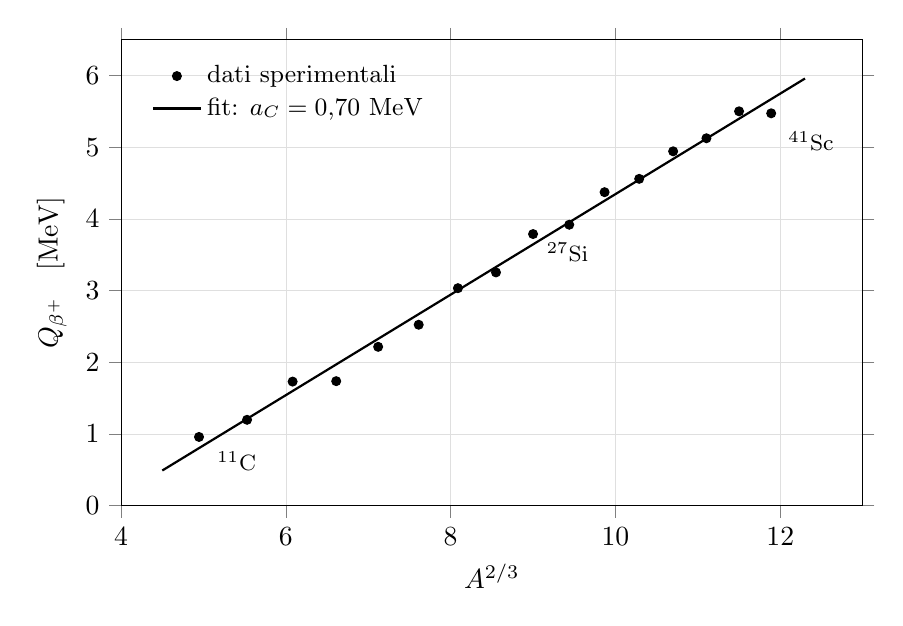
\begin{tikzpicture}
    \begin{axis}[
        width=11cm, height=7.5cm,
        xlabel={$A^{2/3}$},
        ylabel={$Q_{\beta^+}$ \; [MeV]},
        xmin=4, xmax=13, ymin=0, ymax=6.5,
        xtick={4,6,8,10,12}, ytick={0,1,2,3,4,5,6},
        grid=both,
        grid style={line width=0.2pt, draw=gray!25},
        axis lines=box,
        tick align=outside,
        legend pos=north west,
        legend cell align=left,
        legend style={draw=none, fill=none, font=\small},
    ]
    \addplot[only marks, mark=*, mark size=1.6pt, black] coordinates {
     (4.946,0.960) (5.529,1.199) (6.082,1.732) (6.611,1.738)
     (7.120,2.217) (7.612,2.525) (8.088,3.035) (8.550,3.255)
     (9.000,3.790) (9.439,3.920) (9.868,4.374) (10.288,4.560)
     (10.700,4.944) (11.104,5.126) (11.500,5.502) (11.890,5.474)
    };
    \addlegendentry{dati sperimentali}
    \addplot[black, thick, domain=4.5:12.3, samples=2] {0.701*x - 2.663};
    \addlegendentry{fit: $a_C = 0{,}70$ MeV}
    \node[anchor=west, font=\footnotesize] at (axis cs:5.05,0.62) {$^{11}$C};
    \node[anchor=north west, font=\footnotesize] at (axis cs:9.05,3.80) {$^{27}$Si};
    \node[anchor=north west, font=\footnotesize] at (axis cs:11.98,5.35) {$^{41}$Sc};
    \end{axis}
    \end{tikzpicture}
    \caption{$Q$-valore del decadimento $\beta^+$ fra nuclei speculari in funzione di $A^{2/3}$, per le coppie da $A = 11$ ad $A = 41$. La pendenza della retta fornisce il coefficiente coulombiano $a_C$.}
    \label{fig:speculari}
\end{figure}

Dalla pendenza si legge $a_C \simeq 0{,}70 \ \text{MeV}$, e invertendo la definizione di $a_C$ si ricava
%
\begin{equation}
    r_0 = \frac{3}{5}\frac{\alpha \hbar c}{a_C} = \frac{0{,}6 \cdot 1{,}44 \ \text{MeV} \cdot \text{fm}}{0{,}70 \ \text{MeV}} \simeq 1{,}2 \ \text{fm}
\end{equation}
in ottimo accordo con il valore ottenuto per altre vie.\\

Un discorso del tutto analogo si può fare con la cattura elettronica, che converte anch'essa un protone in un neutrone e porta quindi ancora da $Y$ a $X$. Ripetendo il conto a partire da $Q_{EC} = M(Y) + m_e - M(X)$ si trova
%
\begin{equation}
    \Delta B = Q_{EC} + m_n - m_e - m_p
\end{equation}
che differisce dalla \eqref{eq:deltaB_Q} per $2m_e$, come deve essere dato che $Q_{EC} = Q_{\beta^+} + 2m_e$.